\section{Training Monitoring and Visualization}
\label{sec:training_monitoring}
Training Generative Adversarial Networks (GANs) is notoriously unstable, and scalar loss metrics (e.g., Generator Loss vs. Discriminator Loss) often fail to capture the true perceptual quality or mode coverage of the generated distribution.
To address this, we implemented a comprehensive suite of visualization diagnostics that runs concurrently with the validation epochs.
These mechanisms provide granular insights into the model's convergence and its adherence to the physical properties of Radar Sounder (RS) data.

\subsection{Pixel Value Distribution Analysis}
Standard image reconstruction metrics like L1 or L2 norm can be misleading if the generator acts as a \enquote{mean regressor}, producing blurry images that minimize error but lack high-frequency texture.
To detect this behavior, we implemented a \textbf{Pixel Value Distribution Monitor} (see \texttt{src.utils.save\_pixel\_distribution}).
At specific training intervals, the system computes and visualizes the histogram of pixel intensities for the Input (Simulated), Target (Real), and Generated (Fake) batches.

\begin{figure}[htbp]
    \centering
    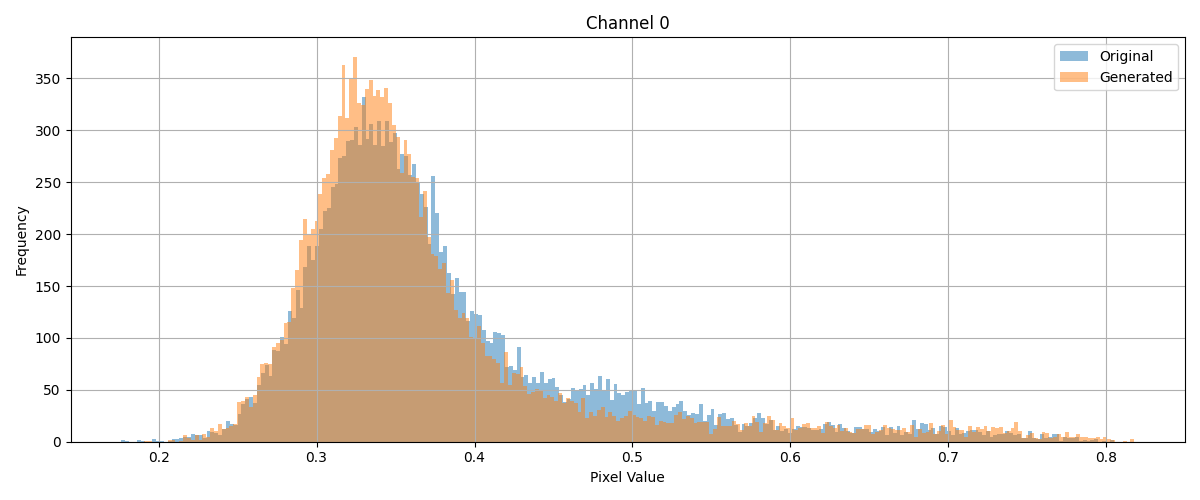
\includegraphics[width=0.9\textwidth]{images/distributions/cg_compare_distribution_5}
    \caption{Example of pixel value distribution comparison. Overlapping the histograms of Real (Target) and Generated data allows for the immediate detection of varying intensity scales or \enquote{mode collapse}, where the generator fails to capture the full dynamic range of the radar signal.}
    \label{fig:pixel_distribution}
\end{figure}

This diagnostic is critical for ensuring that the CycleGAN effectively aligns the \textit{marginal distributions} of the two domains.
A discrepancy in the histogram tails, for instance, often indicates that the model is failing to reproduce the decay characteristic of the Martian surface, or is truncating the noise floor.

\subsection{Range-Line Intensity Profiling}
A unique characteristic of radar sounding data is the physical attenuation of the signal with depth.
To verify that the generator learns this physical law—rather than simply performing style transfer on surface features—we introduced a \textbf{Range-Line Intensity Profile} evaluation (\texttt{src.utils.save\_rangeline\_comparison}).

This routine extracts a 1D vertical slice (A-scan) from the center of the generated radargram and compares it against the corresponding trace from the real target.
By overlaying these profiles, we can visually inspect:
\begin{itemize}
    \item \textbf{Surface Peak Matching:} Whether the generated surface return matches the amplitude and width of the real signal.
    \item \textbf{Attenuation Trend:} Whether the noise floor decays correctly with depth, mirroring the physical loss tangent of the crust. 
\end{itemize}
Discrepancies in the lower sections of this profile were instrumental in identifying the need for additional Z-score normalization in later stages of the pipeline.

\subsection{Evolutionary Trajectory Plotting}
To monitor the temporal stability of the learning process, the framework maintains a fixed \enquote{anchor} sample that is processed at every epoch.
The \texttt{plot\_evolution} module visualizes the trajectory of this specific sample throughout the training timesteps, arranging the snapshots in a chronological grid.
This visualization allows for the detection of \textit{cyclical forgetting}, where the model learns a feature (e.g., a specific speckle pattern) only to unlearn it in subsequent epochs due to the adversarial game's instability.

